%\begin{frame}{Extraction des phrases-clés}
%\og{}\textcolor{deepblue}{Phrases-clés}\fg{}, angl. \textit{keyphrases}
%\begin{itemize}
%\item séquences de plusieurs mots (ex. \textit{sclérose latérale amyotrophique})
%\item reflètent plus précisément le contexte sémantique du texte \\\small{$\neq$ mots-clés, angl. \textit{keywords} : unigrammes de mot (ex. \textit{sclérose})}
%\end{itemize}
%\bigskip
%%\centering
%%Extraction de \og{}phrases-clés\fg{} (angl. \textit{keyphrases})
%%\\~\\
%%\begin{block}{Extraction de phrases-clés}
%%\justifying
%%Processus de \underline{sélection} automatique d'un petit ensemble de phrases les plus pertinentes à partir d'un texte donné \citep{schopf2022}.
%%\end{block}
%%\begin{block}{Prédiction de phrases-clés}
%%\justifying
%%Processus de \underline{génération} des phrases-clés qui résument parfaitement un document donné \citep{xie2023}.
%\begin{columns}[t,onlytextwidth]
%\column{.45\textwidth}
%\textcolor{violet}{Extraction}
%\justifying
%
%Processus de \underline{sélection} automatique d'un petit ensemble de phrases les plus pertinentes à partir d'un texte donné.
%\vspace{-0.2cm}
%\begin{flushright}
%\small{\citep{schopf2022}}
%\end{flushright} 
%\column{.45\textwidth}
%\textcolor{violet}{Prédiction}
%\justifying
%
%Processus de \underline{génération} des phrases-clés qui résument parfaitement un document donné.
%\vspace{0.3cm}
%\begin{flushright}
%\small{\citep{xie2023}}
%\end{flushright}
%\end{columns}%Extraction de phrases-clés
%%
%%Processus de \underline{sélection} automatique d'un petit ensemble de phrases les plus pertinentes à partir d'un texte donné \citep{schopf2022}.
%%
%%\begin{block}{Prédiction de phrases-clés}
%%\justifying
%%Processus de \underline{génération} des phrases-clés qui résument parfaitement un document donné \citep{xie2023}.
%%\end{block} 
%\end{frame}

%\begin{frame}{Extraction des phrases-clés : méthode \texttt{keybert}}
%	\begin{enumerate}
%		\small
%		\item entrée : un document
%		\item tokénisation du document en phrases-clés candidates (PCC)
%		\item génération des plongements du doc. et des PCC par un modèle de langage
%		\item calcul de la similarité cosinus entre le document et les PC
%	\end{enumerate}
%	\begin{figure}
%		\centering
%		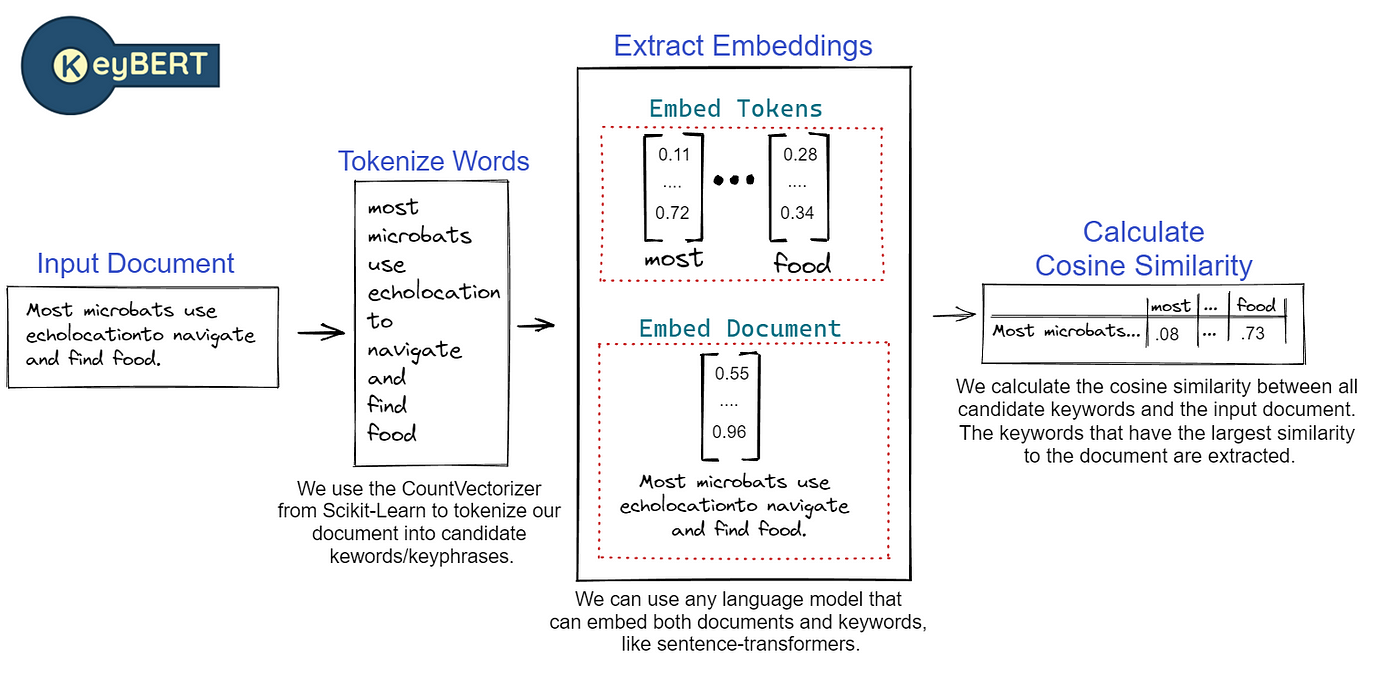
\includegraphics[width=80mm,scale=0.5]{pic/keybert.png}
%		\caption{\textit{Pipeline} de la librairie \texttt{keybert} \citep{grootendorst2020keybert}.}
%		\label{fig:enter-label}
%	\end{figure}
%\end{frame}
%
%\begin{frame}{Extraction des phrases-clés : méthode \textit{PatternRank}\\
%		\quad \quad \quad\ \quad \quad \quad \quad \quad \quad \quad \ \ \ \ \ \small{Librairie \texttt{keyphrase-vectorizers}}}
%	%\begin{itemize}
%	%\item extraction des phrases-clés non-supervisée
%	%\item exploite des modèles de langues pré-entraînés + parties du discours
%	%\end{itemize}
%	\begin{enumerate}
%		\small
%		\item entrée : un seul document texte tokenisé
%		\item étiquetage des tokens avec les balises du partie du discours (POS)
%		\item sélection des tokens selon le motif POS $\rightarrow$ phrases-clés candidates (PCC)
%		\item génération des plongements du doc. et des PCC par un modèle de langue
%		\item calcul des similarités cosinus entre ces deux types de plongements +  \\classement des PCC par ordre décroissant
%		\item extraction des \textit{N} PC les plus représentatives
%	\end{enumerate}
%	\begin{figure}
%		\centering
%		\includegraphics[width=110mm,scale=0.5]{pic/patternrank\_workflow.png}
%		\caption{\textit{Workflow} de la méthode \textit{PatternRank} \citep{schopf2022}.}
%		\label{fig:enter-label}
%	\end{figure}
%	\notecite{schopf2022}
%\end{frame}


